\documentclass[11pt]{article}
\usepackage[margin=1in]{geometry}
\usepackage{amsmath,amssymb}
\usepackage{booktabs}
\usepackage{graphicx}
\usepackage{caption}
\usepackage{subcaption}
\usepackage{hyperref}
\usepackage{xcolor}
\usepackage{microtype}
\usepackage{parskip}
\usepackage{enumitem}
\usepackage{multirow}
\usepackage{array}
\usepackage{tabularx}

\hypersetup{
    colorlinks=true,
    linkcolor=blue!70!black,
    citecolor=blue!70!black,
    urlcolor=blue!70!black,
}

\setlength{\parskip}{0.5em}
\setlength{\parindent}{0pt}

\title{%
    \large\textbf{Evaluating TurboQuant-Family Compression on CLIP Multimodal Embeddings}\\[0.4em]
    \normalsize CS 639: Introduction to Foundation Models, Final Report, Spring 2026
}

\author{%
    aagarwal235 \and
    akumar323 \and
    cajain \and
    rsingh \and
    sagarwal235 \and
    sbarjatya \and
    sdatta9
}

\date{Spring 2026}

\begin{document}
\maketitle

%-----------------------------------------------------------------------
\section{Introduction}

CLIP~\cite{radford2021clip} encodes images and text into a shared 512-dimensional embedding space,
enabling cross-modal retrieval by dot-product similarity. At scale this creates a real storage problem:
a billion-image index at float32 precision requires over 2\,TB before any search infrastructure.
Compressing those embeddings is the natural fix, but most methods either require expensive training or
sacrifice too much retrieval quality. Three recent analytic compressors, QJL~\cite{zandieh2024qjl},
PolarQuant~\cite{han2026polarquant}, and TurboQuant~\cite{zandieh2026turboquant}, are appealing
alternatives: they require no training data, compress near-instantly, and are theoretically near-optimal
for inner-product estimation. If they hold up on CLIP, databases could be compressed 8--30$\times$ with
no index rebuild, making large-scale image search practical on commodity hardware.

The problem is that all three were evaluated only on text embeddings or LLM activations. CLIP embeddings
are geometrically different: image and text vectors occupy systematically offset regions of the unit
sphere, a phenomenon known as the \textit{modality gap}~\cite{liang2022gap}. Cross-modal retrieval
depends on this alignment surviving compression intact, and compressors designed for isotropic
text-like distributions may not preserve it. We implement all three from paper specifications and
evaluate them on CLIP, making this the first study of the TurboQuant family on multimodal embeddings.

\subsection*{Hypotheses}
\textbf{H1:} Cross-modal tasks (text-to-image, image-to-text) will degrade faster under compression than
same-modal tasks (text-to-text, image-to-image), because cross-modal retrieval depends on preserving
inter-modal geometric alignment, which is more fragile than within-modality neighborhood structure.

\textbf{H2:} The analytic compressors can compress CLIP embeddings to 3--4\,bits with acceptable
quality and be competitive with trained FAISS-PQ at 2--4\,bits per dimension.

\subsection*{Research Questions}
\begin{itemize}[leftmargin=*, itemsep=0pt]
  \item How much memory can be saved while keeping Recall@10 within 5\%, 10\%, and 20\% of the uncompressed baseline?
  \item Does cross-modal retrieval degrade faster than same-modal retrieval under the same compression? (\textbf{H1})
  \item Does TurboQuant transfer from text embeddings to CLIP multimodal embeddings? (\textbf{H2})
  \item How do training-free analytic methods compare to FAISS-PQ in the quality-memory tradeoff?
\end{itemize}

%-----------------------------------------------------------------------
\section{Related Work}

\paragraph{CLIP and multimodal retrieval.}
Radford et al.~\cite{radford2021clip} introduced contrastive language-image pretraining, producing joint
embeddings now widely used for cross-modal retrieval. Liang et al.~\cite{liang2022gap} characterized the
modality gap and showed it persists across architectures. Recent work~\cite{yaras2026gap} studies the
robustness implications of the modality gap under naive uniform quantization, motivating our study of
near-optimal quantizers on the same problem.

\paragraph{Product quantization.}
Johnson et al.~\cite{johnson2019faiss} introduced FAISS with product quantization (PQ), which learns
data-specific codebooks. PQ remains the practical standard for large-scale retrieval but requires a
training pass over representative data.

\paragraph{Analytic compressors.}
Zandieh et al.~\cite{zandieh2024qjl} introduced QJL: a random Johnson--Lindenstrauss projection followed
by sign quantization with a provably unbiased inner-product estimator. Han et al.~\cite{han2026polarquant}
introduced PolarQuant, which uses recursive polar coordinates and analytically derived Beta-distribution
angle codebooks requiring no training data. Zandieh et al.~\cite{zandieh2026turboquant} combined both
in TurboQuant, achieving near-optimal distortion at 2.5--3.5 bits per dimension. All three were evaluated
exclusively on text and language model activation vectors.

\paragraph{Community implementations.}
Several open-source projects have implemented TurboQuant since its publication: \texttt{tonbistudio/turboquant-pytorch}~\cite{tonbistudio2026} documents edge cases in QJL residuals, Memoriant's KV-cache benchmark~\cite{memoriant2026} and llama.cpp discussions~\cite{ggmlorg2026} highlight latency overheads at long context lengths, and MLX-VLM~\cite{mlxvlm2026} uses SRHT preconditioning over plain Gaussian projections.
All of these study LLM inference workloads and evaluate only same-modal nearest-neighbor tasks.
None measures whether compression preserves cross-modal alignment, which is the gap this work addresses.

Our setting is similar to prior work in that we use the same compressors and the same inner-product retrieval framework. It differs in two critical ways:
the embedding space is multimodal, and the retrieval tasks are cross-modal. These differences matter because
existing evaluations use same-modal nearest-neighbor benchmarks that cannot detect whether
compression damages inter-modal alignment. FAISS-PQ has not been evaluated alongside the analytic compressors under matched conditions or on cross-modal
tasks. No prior work measures whether the modality gap survives quantization, which is the
central question we address.

%-----------------------------------------------------------------------
\section{Methodology}

We compare three analytic compressors against FAISS-PQ (the standard trained baseline) and float32.
Alternatives such as scalar quantization reduce to special cases of PQ and are not designed for
inner-product estimation. Retrieval is asymmetric (queries at float32, database compressed), matching
real deployment. Recall@10 is preferred over Recall@1 for robustness to near-duplicate captions.
The four-task design (two cross-modal, two same-modal) is the minimal structure to test H1: same-modal
tasks are controls, and any gap between groups isolates cross-modal fragility.

\subsection{Dataset, Embeddings, and Hardware}

We use the Hugging Face parquet mirror of Flickr30k~\cite{young2014flickr}, containing 31{,}014 images
and 155{,}070 captions with five captions per image. Flickr30k provides multi-answer ground truth for
image$\to$text tasks, and its 31k-image scale is large enough to expose quantization artifacts while
remaining tractable for fully CPU-resident experiments. Larger web-crawled datasets such as LAION
would require GPU-scale retrieval infrastructure and introduce noisy paired annotations. We use CLIP ViT-B/32 because it
is the most widely deployed CLIP variant and its 512-dimensional embeddings are a natural target:
large enough to stress compressors across multiple bit-widths, small enough to fit the entire
database in CPU RAM. Images and captions are embedded with frozen CLIP ViT-B/32 into
512-dimensional vectors and L2-normalized to unit norm (required by the polar decomposition
in PolarQuant). All embeddings were computed once on a T4 GPU in Google Colab; all compression, retrieval,
and analysis steps were run on CPU on a MacBook Pro with an M1 Pro chip (16\,GB RAM). This split mirrors
the intended deployment: embedding inference is GPU-bound and done once, while the indexing and retrieval
experiments are fully CPU-resident.

Each uncompressed embedding requires $512 \times 4 = 2{,}048$ bytes. The full image database (31{,}014
vectors) occupies 63.5\,MB; the text database (155{,}070 vectors) occupies 317\,MB.

\subsection{Retrieval Tasks and Metrics}

We evaluate four tasks using Recall@$k$ for $k \in \{1, 5, 10\}$:
\begin{itemize}[itemsep=1pt]
  \item \textbf{T1 text$\to$image (cross-modal):} a caption queries the image database; its paired image is correct.
  \item \textbf{T2 image$\to$text (cross-modal):} an image queries the caption database; any of its five captions counts.
  \item \textbf{T3 text$\to$text (same-modal):} a caption queries the caption database; the other four captions of the same image are correct (self-retrieval excluded).
  \item \textbf{T4 image$\to$image (same-modal):} an image queries the image database; the float32 top-1 image neighbor (excluding the query) is the target.
\end{itemize}

T1 and T2 are the primary stress test. T3 and T4 serve as same-modal controls.
We report Recall@10 as the primary metric: it is less noisy than Recall@1 while still sensitive to
ranking degradation under compression. Queries always remain at full float32 precision; only the database
is compressed (asymmetric retrieval).

\subsection{Compressors and Implementation}

Table~\ref{tab:methods} summarizes the four methods. All three analytic compressors are implemented from
paper specifications without adapting any existing GPU/CUDA code.

\begin{table}[h!]
  \centering
  \caption{Compressors evaluated. All analytic methods are implemented from paper specifications.}
  \label{tab:methods}
  \small
  \begin{tabularx}{\linewidth}{llXl}
    \toprule
    \textbf{Method} & \textbf{Training?} & \textbf{Description} & \textbf{Bits} \\
    \midrule
    Uncompressed & N/A & float32 reference & 32 \\
    QJL          & No  & SRHT preconditioning + sign quantization & 1$^*$ \\
    PolarQuant   & No  & recursive polar transform, analytic codebooks & 1, 2, 4 \\
    TurboQuant   & No  & PolarQuant main stage + 1-bit QJL residual & 1, 2, 4 \\
    FAISS-PQ     & Yes & learned product quantization codebooks & 1, 2, 4, 8 \\
    \bottomrule
    \multicolumn{4}{l}{\footnotesize $^*$ SRHT is a bijection in $d$ dimensions; QJL is capped at 1\,bit/dim.}
  \end{tabularx}
\end{table}

\paragraph{QJL.}
We apply a Subsampled Randomized Hadamard Transform (SRHT) for preconditioning: each database vector is
sign-flipped by a random diagonal $D \in \{-1,+1\}^d$, passed through the fast Walsh--Hadamard transform,
and $m$ coordinates are subsampled. Only the sign of each projected coordinate is stored. The asymmetric
inner-product estimator is:
\[
    \langle q, x \rangle \approx \sqrt{\tfrac{\pi}{2}} \cdot \frac{1}{m}
    \sum_{i=1}^{m} (\mathrm{SRHT}(q))_i \cdot \mathrm{sign}((\mathrm{SRHT}(x))_i) \cdot \|x\|_2.
\]
SRHT whitens CLIP's non-isotropic coordinate distribution so every sign bit is equally informative,
unlike a plain Gaussian projection where low-variance dimensions waste bits.

\paragraph{PolarQuant.}
A shared random orthogonal rotation is applied, then the vector is recursively decomposed into polar
coordinates: at each level, adjacent pairs are converted to a radius and an angle. Level 1 angles cover
$[0, 2\pi]$; deeper levels cover $[0, \pi/2]$ because their inputs are radii (non-negative). We use a
variable bit-width schedule: level 1 gets (\texttt{angle\_bits}+1) bits to cover the full circle, and
deeper levels get $\max(1, \texttt{angle\_bits}-1)$ bits. Codebooks are derived analytically from the
theoretical polar angle PDFs (data-free), following the Beta-distribution derivation in~\cite{han2026polarquant}.

\paragraph{TurboQuant.}
At $b$ total bits/dim, $b-1$ bits go to PolarQuant as the main compression stage, and 1 bit goes to QJL
applied to the residual $r = x - \hat{x}_{\text{polar}}$. Because residuals are not unit-normalized,
QJL uses its full inner-product estimator (with norm scaling), not cosine mode. The final score is:
\[
    \hat{s}(q, x) = \langle q, \hat{x}_{\text{polar}} \rangle + \sqrt{\tfrac{\pi}{2}} \cdot \frac{1}{m}
    \sum_i (\mathrm{SRHT}(q))_i \cdot \mathrm{sign}((\mathrm{SRHT}(r))_i) \cdot \|r\|_2.
\]
At $b=1$, the polar stage has 0 bits and TurboQuant reduces to pure QJL.

\paragraph{FAISS-PQ.}
We use 8-bit codebooks with number of subquantizers $M$ such that $M \cdot 8 / 512$ equals the target
bits per dimension. This gives $M = 64, 128, 256, 512$ for 1, 2, 4, 8\,bits/dim respectively.

\subsection{Bit-Widths, Seeds, and Validation}

We evaluate bit budgets $\{1, 2, 4\}$ for the analytic methods and $\{1, 2, 4, 8\}$ for FAISS-PQ, with
float32 as the uncompressed baseline. Each configuration is run over five random seeds (0--4) to account
for randomness in projections, rotations, and codebook initialization; we report seed means with standard
deviation as error bars. Before running CLIP experiments, we validated all compressors on synthetic unit
vectors, confirming that inner-product correlation with ground truth improves monotonically with
bit-width across all methods.

%-----------------------------------------------------------------------
\section{Implementation: From V1 to V2}
\label{sec:v1v2}

V1 was functional but deviated from the papers in three ways. All results in this paper use the
revised V2 implementation.

\paragraph{QJL: Gaussian projection $\to$ SRHT.}
CLIP coordinates are non-isotropic (image kurtosis $\approx 69$), so a Gaussian projection wastes
sign bits on low-variance dimensions. V2 uses SRHT, which whitens the distribution before subsampling.
This alone improves R@1 from 0.67 to 0.90 at 1-bit and cuts encoding from $O(md)$ to $O(d\log d)$.

\paragraph{PolarQuant: empirical codebooks $\to$ analytic codebooks.}
V1 fitted Lloyd-Max codebooks on CLIP data; V2 derives them from theoretical polar angle PDFs
(data-free) and gives the first recursion level one extra bit since its angles span $[0,2\pi]$
vs.\ $[0,\pi/2]$ at deeper levels. Cross-modal Recall@10 at 2\,bits improves from 0.349 to 0.406
(T1) and 0.548 to 0.629 (T2).

\paragraph{TurboQuant: MSE stage $\to$ PolarQuant stage.}
V1's TurboQuantMSE stage (Cartesian scalar quantization) is not suited to unit-normalized embeddings;
at 2\,bits, TurboQuant scored below its own components. V2 replaces it with PolarQuant, matching
Algorithm 2 of~\cite{zandieh2026turboquant}, and fixes two subtleties: residuals require norm
scaling (\texttt{cosine=False}), and the two stages need independent seeds. The result is +104\% on
T1 (0.157 $\to$ 0.321) and +100\% on T2 (0.263 $\to$ 0.525) at 2\,bits.

\paragraph{Summary.} Table~\ref{tab:v1v2} shows the gains across all three compressors at 2\,bits/dim.

\begin{table}[h!]
  \centering
  \caption{V1 vs.\ V2 Recall@10 at 2\,bits/dim on cross-modal tasks. All V2 numbers are used throughout this report.}
  \label{tab:v1v2}
  \small
  \begin{tabular}{lcccc}
    \toprule
    \textbf{Method} & \textbf{Version} & \textbf{T1 txt$\to$img} & \textbf{T2 img$\to$txt} & \textbf{Mean (all tasks)} \\
    \midrule
    \multirow{2}{*}{QJL (1-bit cap)}
      & V1 (Gaussian) & 0.154 & 0.255 & --- \\
      & V2 (SRHT)     & 0.233 & 0.385 & --- \\
    \midrule
    \multirow{2}{*}{PolarQuant}
      & V1 (empirical codebooks) & 0.349 & 0.548 & 0.599 \\
      & V2 (analytic codebooks)  & 0.406 & 0.629 & 0.638 \\
    \midrule
    \multirow{2}{*}{TurboQuant}
      & V1 (MSE stage + Gaussian QJL) & 0.157 & 0.263 & 0.387 \\
      & V2 (PolarQuant stage + SRHT QJL) & 0.321 & 0.525 & 0.584 \\
    \bottomrule
  \end{tabular}
\end{table}

%-----------------------------------------------------------------------
\section{Results}

\subsection{Main Retrieval Results}

Table~\ref{tab:retention} reports Recall@10 \textit{retention} (the fraction of uncompressed
Recall@10 that each method preserves), averaged over five seeds. Uncompressed baselines are:
T1 = 0.498, T2 = 0.741, T3 = 0.528, T4 = 1.000.

\begin{table}[h!]
  \centering
  \caption{Recall@10 retention (as \% of uncompressed baseline), averaged over 5 seeds and 1{,}000 queries per task. Values $\geq 95\%$ are \textbf{bold}; values $< 70\%$ are \textit{italic}.}
  \label{tab:retention}
  \small
  \begin{tabular}{llccccc}
    \toprule
    \textbf{Method} & \textbf{Bits} & \textbf{T1 txt$\to$img} & \textbf{T2 img$\to$txt} & \textbf{T3 txt$\to$txt} & \textbf{T4 img$\to$img} & \textbf{Mean} \\
    \midrule
    Uncompressed & 32 & 100\% & 100\% & 100\% & 100\% & 100\% \\
    \midrule
    FAISS-PQ & 1 & \textit{67.7\%} & \textit{65.9\%} & 77.1\% & 85.1\% & 75.3\% \\
    FAISS-PQ & 2 & 94.0\% & 90.8\% & 94.5\% & 97.1\% & 94.4\% \\
    FAISS-PQ & 4 & \textbf{99.0\%} & \textbf{99.3\%} & \textbf{99.4\%} & \textbf{99.4\%} & \textbf{99.3\%} \\
    \midrule
    QJL$^*$ & 1 & \textit{46.8\%} & \textit{51.9\%} & 95.3\% & 91.6\% & 73.6\% \\
    \midrule
    PolarQuant & 1 & \textit{63.7\%} & \textit{68.3\%} & 97.5\% & 97.0\% & 83.4\% \\
    PolarQuant & 2 & 81.5\% & 84.9\% & 98.9\% & 99.5\% & 91.2\% \\
    PolarQuant & 4 & \textbf{98.4\%} & 98.1\% & \textbf{100\%} & \textbf{100\%} & \textbf{99.1\%} \\
    \midrule
    TurboQuant & 1 & \textit{46.8\%} & \textit{51.9\%} & 95.3\% & 91.6\% & 73.6\% \\
    TurboQuant & 2 & \textit{64.5\%} & 70.9\% & 97.9\% & 97.6\% & 84.6\% \\
    TurboQuant & 4 & 94.6\% & \textbf{95.7\%} & \textbf{99.6\%} & \textbf{100\%} & \textbf{97.7\%} \\
    \midrule
    \multicolumn{7}{l}{\footnotesize $^*$ QJL with SRHT is structurally capped at 1\,bit/dim; higher bit-widths were not evaluated.}
  \end{tabular}
\end{table}

\paragraph{H1: Cross-modal fragility (strongly confirmed).}
Figure~\ref{fig:retention} shows the clearest result: same-modal tasks (T3, T4) stay above 91\% retention
even at 1\,bit/dim, while cross-modal tasks (T1, T2) drop to 47--68\% at the same budget. The asymmetry
holds for every compressor. The cause is geometric: the modality gap (cosine between mean image and text
embeddings = 0.344, gap norm $\approx 0.80$) is larger than typical within-modality distances, and
orthogonal rotations preserve it. A perturbation small enough to stay within one modality's neighborhood
can still cross the inter-modal boundary.

\paragraph{H2: TurboQuant transfer (supported, with a caveat).}
TurboQuant works on CLIP and improves with each added bit. At 4\,bits it retains 94.6\%/95.7\% of
cross-modal recall (T1/T2), close to PolarQuant (98.4\%/98.1\%) and FAISS-PQ (99\%). It does not beat
PolarQuant at any bit-width because it always reserves 1 bit for the QJL residual, leaving only $b{-}1$
bits for the polar stage. At $b{=}1$ it reduces to pure QJL; at $b{=}2$ the polar codebook has just 2
entries. It pays off at 4\,bits and is substantially better than QJL alone (+25--48 points on T1 at
2--4 bits).

\begin{figure}[t!]
  \centering
  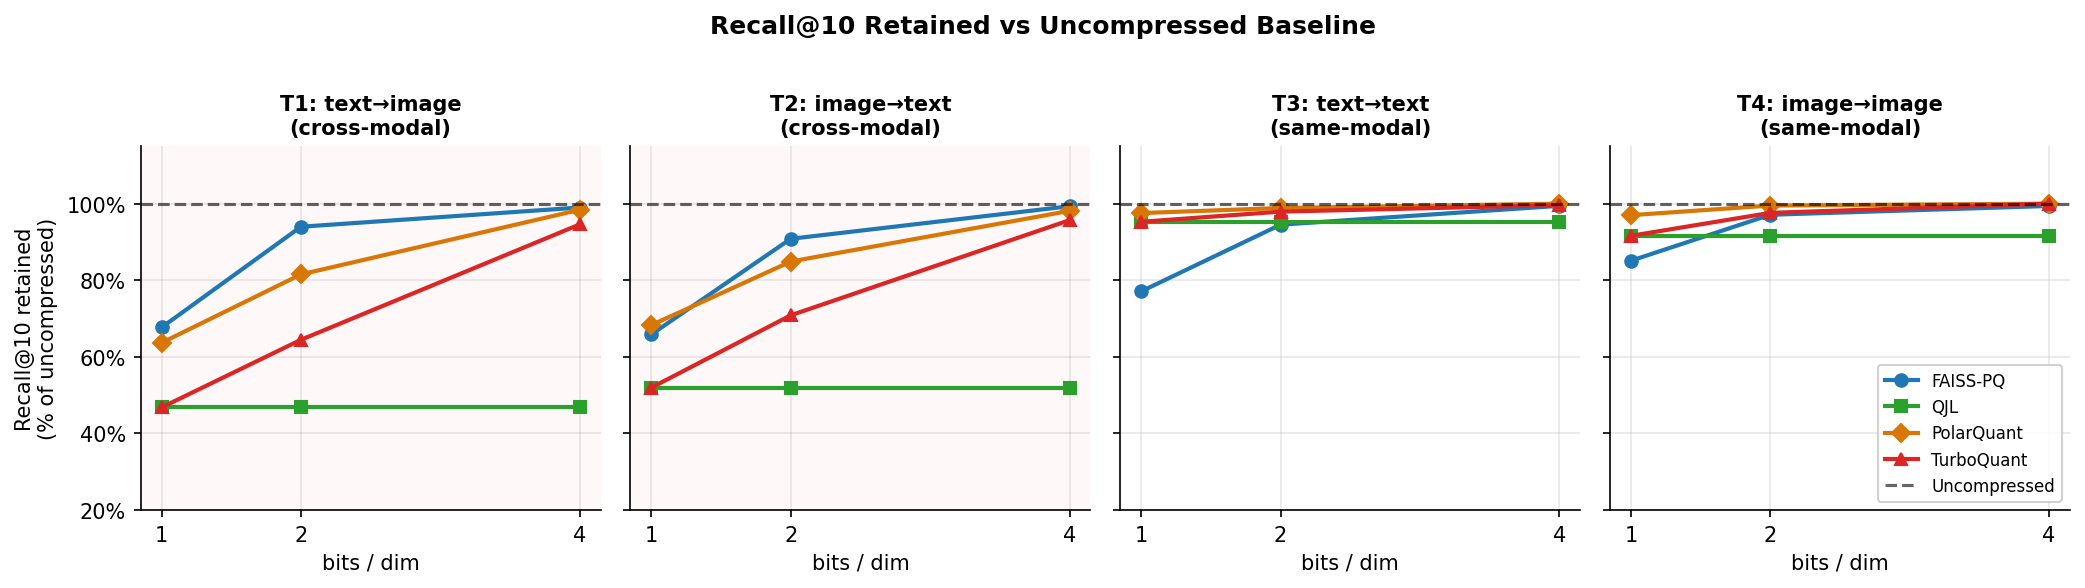
\includegraphics[width=\linewidth]{figs2/fig1_retention_all_tasks}
  \caption{Recall@10 retention (\% of uncompressed) vs.\ bits/dim for all four tasks.
  Cross-modal panels (T1, T2) shown on a red-tinted background. Same-modal tasks (T3, T4)
  stay near 100\% even at 1\,bit/dim; cross-modal tasks drop sharply at low bit budgets.
  Error bars are standard deviations across five seeds.}
  \label{fig:retention}
\end{figure}

\subsection{Memory, Efficiency, and Geometry}

\paragraph{Memory-accuracy tradeoff.}
Figures~\ref{fig:memory_accuracy} and~\ref{fig:savings_recall} show the Pareto frontier and the
cross-modal vs.\ same-modal split. At 4\,bits, PolarQuant (260\,B) essentially matches FAISS-PQ (256\,B)
with no training. At 2\,bits, FAISS-PQ (128\,B) is the only method above 90\% cross-modal retention;
PolarQuant (136\,B) reaches 80\%. For target thresholds, Figure~\ref{fig:threshold} confirms that
$\geq$95\% cross-modal retention requires 4\,bits from either FAISS-PQ or PolarQuant. Storage costs per
vector: FAISS-PQ 64--256\,B, QJL 68\,B (fixed), PolarQuant 72--260\,B, TurboQuant 136--328\,B across
1--4 bits, vs.\ 2{,}048\,B uncompressed.

\begin{figure}[t!]
  \centering
  \begin{subfigure}[b]{0.49\linewidth}
    \centering
    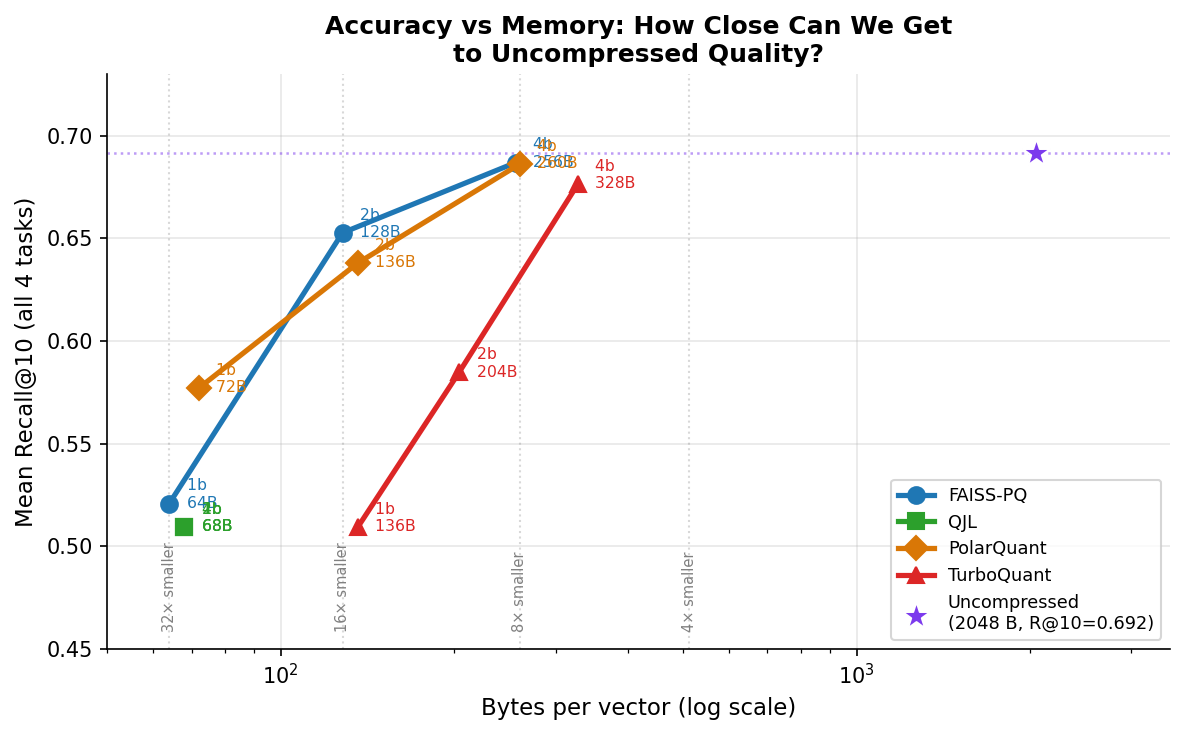
\includegraphics[width=\linewidth]{figs2/fig2_accuracy_vs_memory}
    \caption{Mean Recall@10 vs.\ bytes/vector.}
    \label{fig:memory_accuracy}
  \end{subfigure}
  \hfill
  \begin{subfigure}[b]{0.49\linewidth}
    \centering
    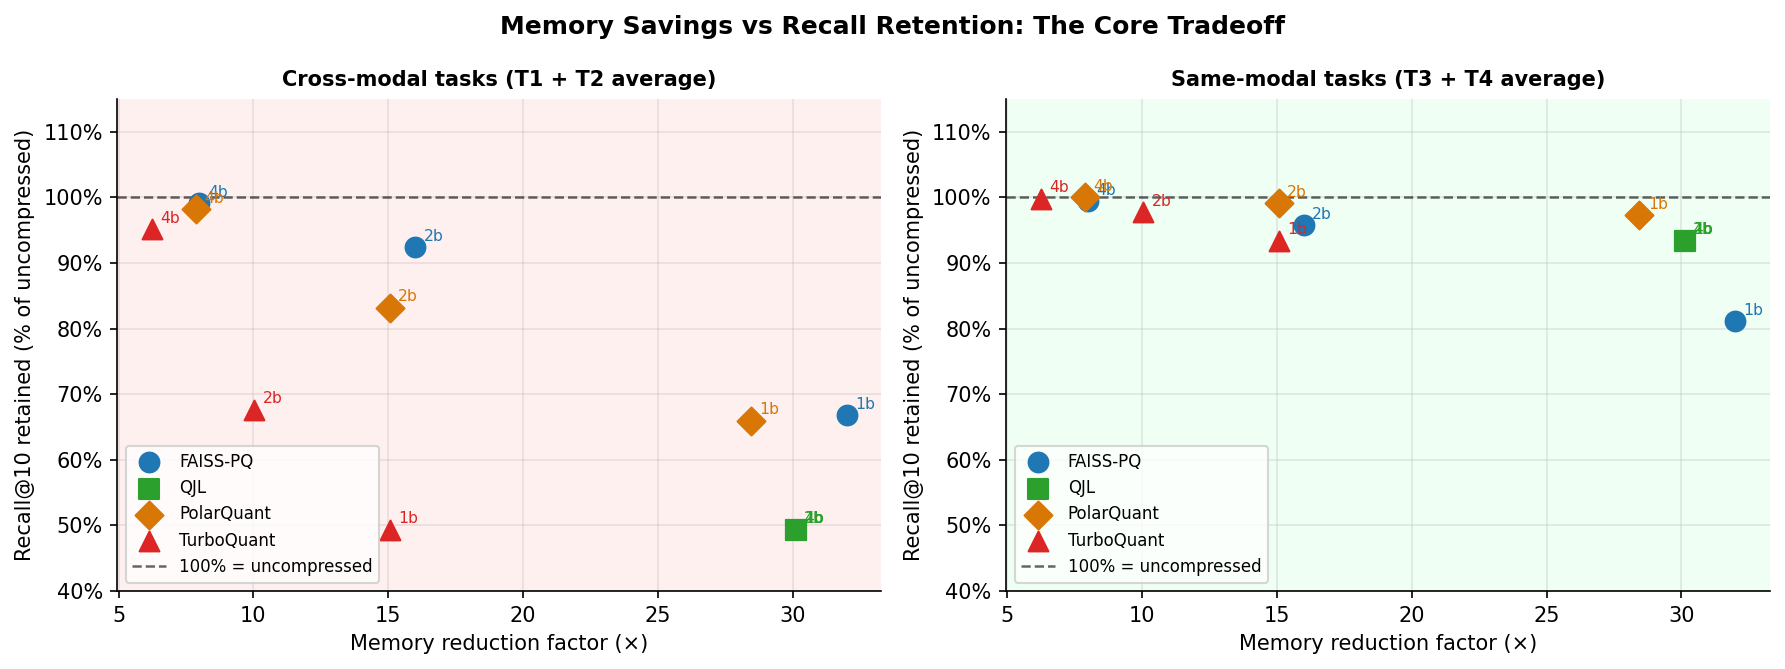
\includegraphics[width=\linewidth]{figs2/fig3_savings_vs_recall}
    \caption{Memory reduction vs.\ recall retention by task type.}
    \label{fig:savings_recall}
  \end{subfigure}
  \caption{Left: PolarQuant and FAISS-PQ converge at 260--256\,B (8$\times$ reduction). Right: cross-modal recall degrades far faster than same-modal recall; at 30$\times$ compression, cross-modal drops to 47--68\% while same-modal stays above 91\%.}
\end{figure}

\begin{figure}[t!]
  \centering
  \begin{subfigure}[b]{0.49\linewidth}
    \centering
    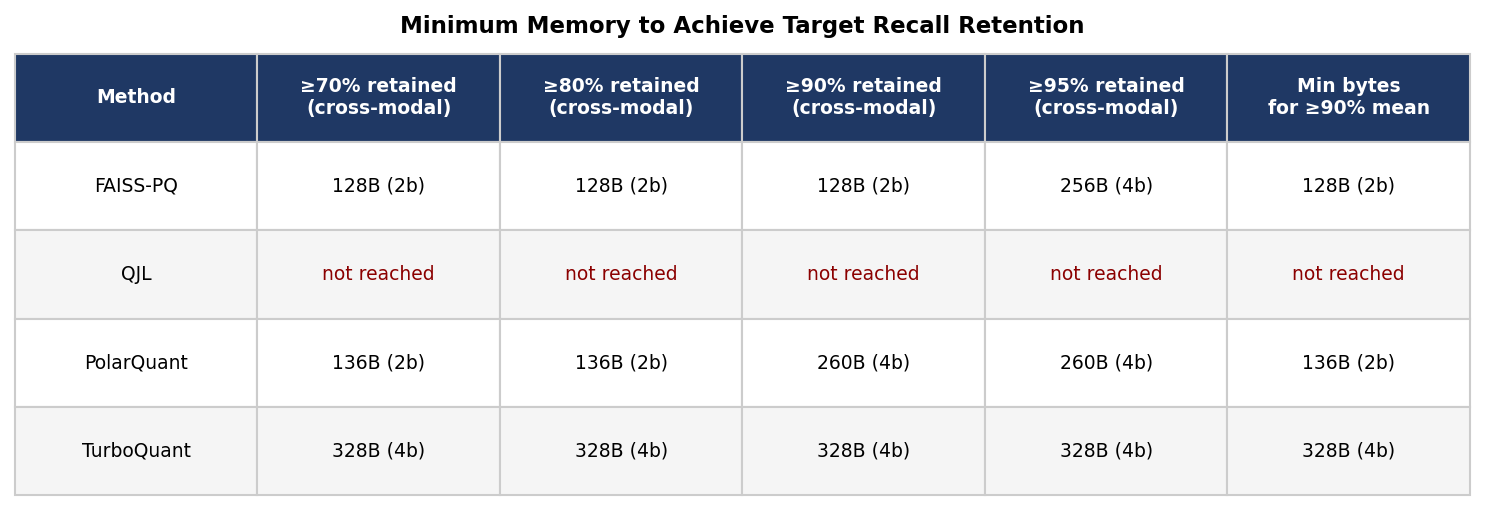
\includegraphics[width=\linewidth]{figs2/fig5_memory_threshold}
    \caption{Min.\ bytes to hit target cross-modal retention.}
    \label{fig:threshold}
  \end{subfigure}
  \hfill
  \begin{subfigure}[b]{0.49\linewidth}
    \centering
    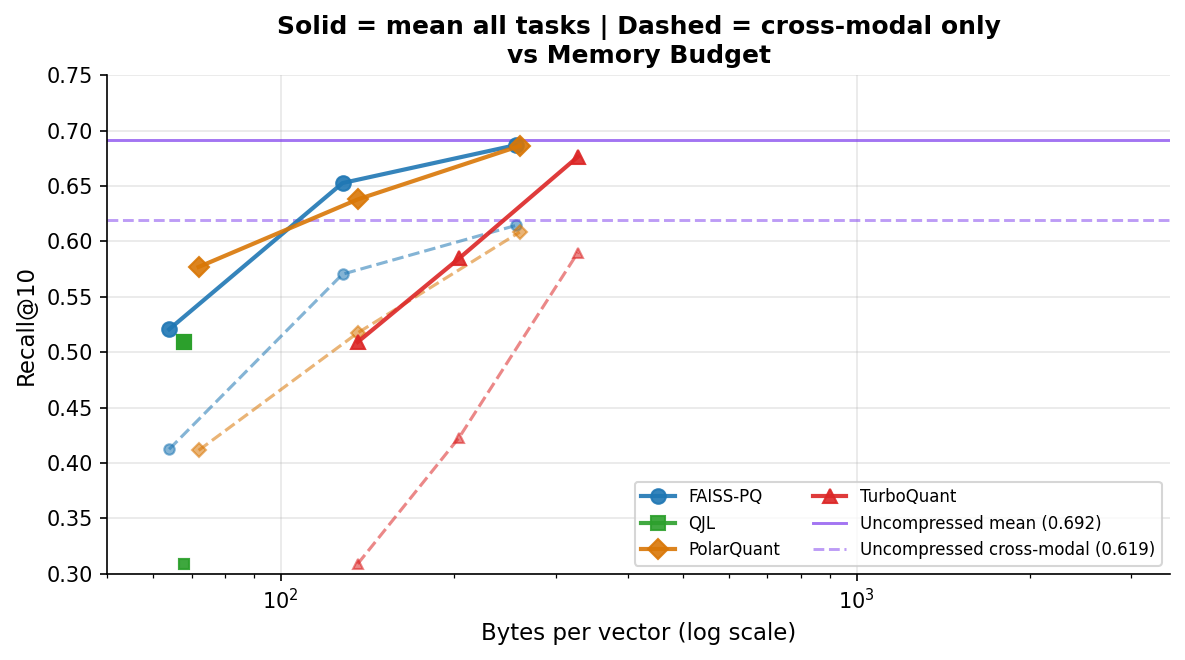
\includegraphics[width=\linewidth]{figs2/fig4_mean_vs_crossmodal}
    \caption{Mean vs.\ cross-modal Recall@10 per method.}
    \label{fig:crossmodal_gap}
  \end{subfigure}
  \caption{Left: only FAISS-PQ and PolarQuant at 4\,bits reach $\geq$95\% cross-modal retention. Right: the gap between mean and cross-modal recall quantifies how much cross-modal tasks are disproportionately hurt; FAISS-PQ shows the smallest gap because its codebooks are data-aware.}
\end{figure}

\paragraph{Efficiency.}
Analytic methods compress 31k vectors in under 0.6 seconds; FAISS-PQ needs 12--17 seconds for codebook
training. Query latency also drops under compression: 1.4--8.7\,ms versus 18.2\,ms for float32.
Figure~\ref{fig:efficiency} shows compression time versus memory savings.

\begin{figure}[t!]
  \centering
  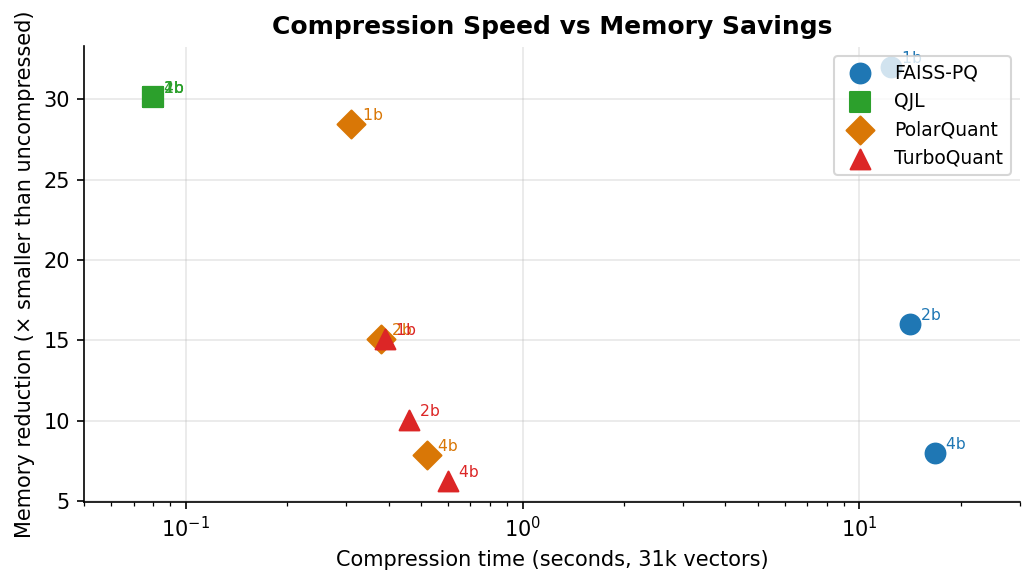
\includegraphics[width=0.7\linewidth]{figs2/fig6_comptime_vs_savings}
  \caption{Compression time (31k vectors) vs.\ memory savings. Analytic methods finish in under 0.6\,s at all bit-widths; FAISS-PQ requires 12--17\,s for codebook training.}
  \label{fig:efficiency}
\end{figure}

\paragraph{Embedding geometry.}
Raw CLIP coordinates are far from Gaussian (image kurtosis $\approx 69$, text $\approx 37$). Random
orthogonal rotation brings both close to zero kurtosis, which validates the theoretical angle PDFs used
by PolarQuant and TurboQuant. Rotation preserves all distances and angles, including the modality gap,
which is why it helps with quantizer design but cannot fix the cross-modal fragility problem.

%-----------------------------------------------------------------------
\section{Discussion}

FAISS-PQ leads at low bit budgets because it knows the data. At 1--2\,bits there are so few bits that
every one needs to capture dataset-specific structure, and a codebook trained on the actual CLIP
distribution does this better than any data-oblivious method. The tradeoff is a training pass and the
need for representative data upfront. If you can afford that, FAISS-PQ is the right call.

PolarQuant performs surprisingly well without any training. Two things explain it. Random orthogonal
rotation brings CLIP's non-Gaussian coordinate distribution close to the angle distributions that
PolarQuant's codebooks are derived for. On top of that, polar decomposition is naturally suited to unit
vectors: angles and radii are a meaningful parameterization for points on the sphere. The analytic
codebooks actually beat our initial empirically fitted ones---V1 to V2 gained +16\% on T1---which
suggests the theoretical priors are a better match for this data than fitting directly to CLIP.

TurboQuant does not beat PolarQuant, and the reason is structural. At moderate bit budgets (2--4\,bits),
the 1-bit overhead for the QJL residual costs more than the correction gains back. At 4\,bits,
PolarQuant already reconstructs most of the signal, so the residual QJL is correcting is tiny---but
QJL still spends one full bit per dimension on it, and that added variance shows up as rank perturbations
in cross-modal retrieval. Retrieval is a ranking problem, not an MSE problem. A small unbiased
correction that also adds variance can hurt top-$k$ rankings even when it improves mean squared error.

\paragraph{Practical guidance.}
Table~\ref{tab:practical} gives a quick reference for choosing a method given a target quality level.

\begin{table}[h!]
  \centering
  \caption{Practical guidance: target retention, recommended method, and cost.}
  \label{tab:practical}
  \small
  \begin{tabularx}{\linewidth}{lllcX}
    \toprule
    \textbf{Target retention} & \textbf{Best method} & \textbf{Bytes/vec} & \textbf{Reduction} & \textbf{Notes} \\
    \midrule
    $\geq 99\%$ & FAISS-PQ & 256\,B & 8$\times$ & Requires training data \\
    $\geq 98\%$ & PolarQuant & 260\,B & 8$\times$ & Training-free \\
    $\geq 90\%$ & FAISS-PQ & 128\,B & 16$\times$ & Requires training data \\
    $\geq 80\%$ & PolarQuant & 136\,B & 15$\times$ & Training-free \\
    $\geq 65\%$ & PolarQuant / TurboQuant & 72--204\,B & 10--28$\times$ & Aggressive regime \\
    Any (instant) & PolarQuant & 72--260\,B & 8--28$\times$ & Best training-free option \\
    \bottomrule
  \end{tabularx}
\end{table}

The short version: 8$\times$ compression with near-lossless cross-modal recall is achievable today.
Each additional factor of 2 in memory savings costs roughly 6--9 percentage points of cross-modal
recall; 30$\times$ compression costs 35+ points.

%-----------------------------------------------------------------------
\section{Limitations}

\textbf{Implementation fidelity.} While our V2 implementations are substantially closer to the paper
descriptions than V1, exact replication is future work. Our PolarQuant uses a PDF-discretized Lloyd-Max
iteration rather than the paper's closed-form Beta CDF inversion. Our TurboQuant reconstructs residuals
explicitly rather than using a lookup-table-based estimator. Both likely understate the theoretical
paper-optimal performance.

\textbf{QJL multi-bit constraint.} The SRHT dimension cap ($m \leq d$) prevents QJL from using bit
budgets above 1\,bit/dim. A Gaussian projection at $m > d$ could unlock multi-bit QJL at the cost of
higher memory and compute.

\textbf{Single backbone and dataset.} We evaluate CLIP ViT-B/32 (512-dim) on Flickr30k. Larger CLIP
models (ViT-L/14, 768-dim; ViT-H/14, 1024-dim) may show different compression behavior due to different
embedding geometry and potentially larger modality gaps. Specialized domains (medical imaging, product
search) may have different cross-modal sensitivity.

\textbf{Reference implementation only.} Our code is a NumPy/CPU reference intended for correctness and
comparison, not a fused GPU or SIMD implementation. Production latency numbers would require packed bit
representations and kernel-level fusion.

%-----------------------------------------------------------------------
\section{Conclusion}

We evaluated QJL, PolarQuant, TurboQuant, and FAISS-PQ on 512-dimensional CLIP ViT-B/32 embeddings of
Flickr30k. The main finding is that cross-modal retrieval degrades far faster under compression than
same-modal retrieval---by a factor of 10--12$\times$ at 1\,bit/dim. This is not a quirk of any
particular compressor; it is a property of CLIP's geometry. The modality gap survives rotation, and
quantization noise that is negligible within a modality can still cross the inter-modal boundary.

Among the methods we tested, FAISS-PQ and PolarQuant are the strongest at 2--4\,bits. If training data
or a codebook rebuild when the database changes is not feasible, PolarQuant is the best available option:
it matches FAISS-PQ at 4\,bits and reaches 80\% cross-modal retention at 2\,bits without seeing a single
data point. TurboQuant reaches 95\% cross-modal retention at 4\,bits and is fully functional, but its
1-bit QJL overhead makes it less efficient at lower bit budgets.

The V1-to-V2 iteration was probably the most instructive part of this project. Going from the MSE stage
to PolarQuant in TurboQuant, and from Gaussian projection to SRHT in QJL, doubled cross-modal recall at
2\,bits with no hyperparameter search. All of that gain came from closer implementation fidelity to the
papers---analytic codebooks, correct angle domains, proper seed splitting. Getting the algorithm right
mattered far more than any tuning we could have done on top of V1.

Future work could test larger CLIP backbones (ViT-L/14, ViT-H/14), add packed bit kernels for
production-speed retrieval, and explore whether allocating different bit budgets to image versus text
embeddings can protect the modality gap more directly.

%-----------------------------------------------------------------------
\bibliographystyle{plain}
\begin{thebibliography}{99}

\bibitem{radford2021clip}
A.~Radford et al.
\newblock Learning transferable visual models from natural language supervision.
\newblock In \textit{ICML}, 2021.

\bibitem{zandieh2026turboquant}
A.~Zandieh, M.~Daliri, M.~Hadian, and V.~Mirrokni.
\newblock {TurboQuant}: Online vector quantization with near-optimal distortion rate.
\newblock In \textit{ICLR}, 2026. arXiv:2504.19874.

\bibitem{zandieh2024qjl}
A.~Zandieh, M.~Daliri, and I.~Han.
\newblock {QJL}: 1-bit quantized {JL} transform for {KV} cache quantization with zero overhead.
\newblock In \textit{AAAI}, 2025. arXiv:2406.03482.

\bibitem{han2026polarquant}
I.~Han, P.~Kacham, A.~Karbasi, V.~Mirrokni, and A.~Zandieh.
\newblock {PolarQuant}: Quantizing {KV} caches with polar transformation.
\newblock In \textit{AISTATS}, 2026. arXiv:2502.02617.

\bibitem{liang2022gap}
W.~Liang et al.
\newblock Mind the gap: Understanding the modality gap in multi-modal contrastive representation learning.
\newblock In \textit{NeurIPS}, 2022.

\bibitem{yaras2026gap}
Y.~Yaras et al.
\newblock Is the modality gap a bug or a feature? A robustness perspective.
\newblock arXiv:2603.29080, 2026.

\bibitem{johnson2019faiss}
J.~Johnson, M.~Douze, and H.~J{\'e}gou.
\newblock Billion-scale similarity search with {GPU}s.
\newblock \textit{IEEE Trans.\ Big Data}, 2019.

\bibitem{young2014flickr}
P.~Young, A.~Lai, M.~Hodosh, and J.~Hockenmaier.
\newblock From image descriptions to visual denotations: New similarity metrics for semantic inference over event descriptions.
\newblock \textit{TACL}, 2014.

\bibitem{tonbistudio2026}
tonbistudio.
\newblock {turboquant-pytorch}: From-scratch {PyTorch} implementation of {TurboQuant}.
\newblock \url{https://github.com/tonbistudio/turboquant-pytorch}, 2026.

\bibitem{memoriant2026}
Memoriant.
\newblock {DGX Spark KV} cache benchmark.
\newblock \url{https://github.com/Memoriant/dgx-spark-kv-cache-benchmark}, 2026.

\bibitem{ggmlorg2026}
ggml-org.
\newblock {TurboQuant}: Extreme {KV} cache quantization discussion.
\newblock \url{https://github.com/ggml-org/llama.cpp/discussions/20969}, 2026.

\bibitem{mlxvlm2026}
Blaizzy.
\newblock {mlx-vlm TurboQuant} reference implementation.
\newblock \url{https://github.com/Blaizzy/mlx-vlm}, 2026.

\end{thebibliography}

%-----------------------------------------------------------------------
\appendix

\section{Use of LLM Assistance}
\label{app:llm}


\begin{enumerate}[leftmargin=*, itemsep=1em]
  \item \textbf{Prompt:} Can you give me a brief but complete summary of the key implementation details for QJL, PolarQuant, and TurboQuant? For each method, just cover the core algorithmic idea, what makes it work.

  \item \textbf{Prompt:} Analyze the code present in the two folders, For each of QJL, PolarQuant, and TurboQuant, I have two implementations, a V1 and a V2. What are the key differences between them, write a brief summary explaining the difference and improvements while using V2?

  \item \textbf{Prompt:} Here are links to a few implementations of TurboQuant: tonbistudio/turboquant-pytorch, Memoriant's DGX Spark KV-cache benchmark, the llama.cpp discussion, and the MLX-VLM reference. Go through each one and tell me what they are doing differently from the original paper, are they changing the projection or the residual stage, or something else? And does any of it apply to our CLIP retrieval setting?

\end{enumerate}

\end{document}
